\documentclass{article}
\usepackage{amsmath}
\usepackage{tikz}

\begin{document}
	
	\title{Nonlinear Heat Conduction Problem}
	\author{}
	\date{}
	\maketitle
	
		\paragraph{Problem Schematic}
	\begin{center}
		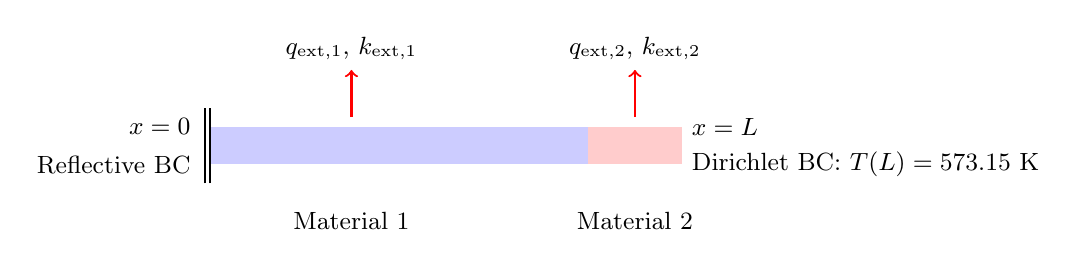
\begin{tikzpicture}[scale=1.2]
			% Draw the domain boundary
			\draw[thick] (0,0) -- (5,0); 
			
			% Material 1 region
			\fill[blue!20] (0,0.2) rectangle (4,-0.2);
			\node[below] at (1.5,-0.6) {\small Material 1};
			
			% Material 2 region
			\fill[red!20] (4,0.2) rectangle (5,-0.2);
			\node[below] at (4.5,-0.6) {\small Material 2};
			
			% Labels for domain boundaries
			\node[left] at (-0.1,0.2) {\small $x=0$};
			\node[right] at (5,0.2) {\small $x=L$};
			
			% Reflective boundary at x=0
			\draw[thick] (0, -0.4) -- (0.0, 0.4);
			\draw[thick] (-0.05, -0.4) -- (-0.05, 0.4);
			\node[left] at (-0.1, -0.2) {\small Reflective BC};
			
			% Dirichlet boundary at x=L
			\node[right] at (5.0, -0.2) {\small Dirichlet BC: $T(L) = 573.15$ K};
			
			% Heat sources
			\draw[->, thick, red] (1.5,0.3) -- (1.5,0.8);
			\node[above] at (1.5, 0.8) {\small $q_{\text{ext},1}$, $k_{\text{ext},1}$};
			
			\draw[->, thick, red] (4.5,0.3) -- (4.5,0.8);
			\node[above] at (4.5, 0.8) {\small $q_{\text{ext},2}$, $k_{\text{ext},2}$};
			
		\end{tikzpicture}
	\end{center}
	
	
	\paragraph{Problem Setup:}
	We consider a \textbf{nonlinear heat conduction problem} defined over a 1D domain with spatial coordinate \( x \), where the system consists of different material properties and external heat sources.
	
	\paragraph{Governing Equation}
	The heat conduction is governed by the nonlinear steady-state heat equation:
	
	\begin{equation}
		\frac{d}{dx} \left( k(T) \frac{dT}{dx} \right) + q_{\text{ext}}(T) = 0, \quad x \in [0, 0.5]
	\end{equation}
	
	where:
	\begin{itemize}
		\item \( T(x) \) is the temperature distribution,
		\item \( k(T) \) is the thermal conductivity, which varies with the length and temperature,
		\item \( q_{\text{ext}}(T) \) represents the external heat source, which also varies with the length and temperature.
	\end{itemize}
	
	\paragraph{Material and Heat Source Properties}
	We define two different materials in the domain with the following properties:
	
	\subparagraph{Thermal Conductivity}
	\begin{enumerate}
		\item First material ($0\leq x\leq0.4$):
		\begin{equation}
			k_1(T) = 16 + \mu + \frac{2150}{T - 73.15}
		\end{equation}
		\item Second material ($0.4\leq x\leq0.5$):
		\begin{equation}
			k_2(T) = 30 + \mu + 2.09 \times 10^{-2} T - 1.45 \times 10^{-5} T^2 + 7.67 \times 10^{-9} T^3
		\end{equation}
	\end{enumerate}
	
	\subparagraph{External Heat Source}
	\begin{enumerate}
		\item First material ($0\leq x\leq0.4$):
		\begin{equation}
			q_{\text{ext},1} = \beta + 35000 + \frac{T}{10}
		\end{equation}
		\item Second material ($0.4\leq x\leq0.5$):
		\begin{equation}
			q_{\text{ext},2} = 10\beta + 5000
		\end{equation}
	\end{enumerate}
	
	\paragraph{Boundary Conditions}
	The system is subject to the following boundary conditions:
	\begin{itemize}
		\item \textbf{At \( x = 0 \) (left boundary):} Reflective (insulating) boundary condition
		\begin{equation}
			\frac{dT}{dx} = 0 \quad \text{at} \quad x = 0
		\end{equation}
		\item \textbf{At \( x = 0.5 \) (right boundary):} Dirichlet condition
		\begin{equation}
			T(0.5) = 573.15 \text{ K} \quad (300^\circ C)
		\end{equation}
	\end{itemize}
	
	\paragraph{Objective}
	The goal is to solve for the steady-state temperature distribution \( T(x) \) for different parameter values associated with nonlinear material properties and external heat sources.
	

\end{document}
